\section{Movement Model}
A movement model describes how an entity moves through space given control input. It consists of internal parameters such as velocities and accelerations. Control input could be a direction of movement supplied by a human using a gamepad, or longer paths supplied by a game engine AI system.

We have not seen any formal description of the movement model. Ususally some ad hoc newtonian physics concepts are combined with springs and animation curves to control the system.

In the following we limit the description to locomotion in the plane. 

We parameterize the movement model as $\mathcal{M}=L,T$ where $L=l_0 \ldots l_n$ is a set of locomotion modes and $\mathcal{I}=i_0 \ldots i_m$ is a set of interpolators that describes the transition between locomotion modes. A movement model defines the behaviour of an actor $\mathcal{A}=\boldsymbol{\omega},p,\dot{p},r,\dot{r}$ where $p$ and $r$ describe position, orientation and their derivatives.  $\boldsymbol{\omega}=\omega_0 \ldots \omega_n$ contains contribution weights for $l \in \mathcal{L}$. Notice $||\vec{\boldsymbol{\omega}}||^2=1$ and usually only a couple of modes will be active as in a transition between walking and running where $\boldsymbol{\omega}=\omega_{walk}:0.8, \omega_{run}:{0.2}, \omega_{other}:0$

An actor is moved with a control signal $\mathcal{C}=l_c, u, \Delta{t}_c, p_c,r_c$ containing locomotion mode, interpolation weight, timestep and target position and orientation respectively. The sparsity of the control signal ilustrates an inherent uncertainty in character animation, as we are challenged to infer a detailed path of movement through often complex environements given a very limited disambiguation or hints to the desired trajectory [Holden A deep learning ...]. We notice that a sampling of the immediate sorroundings could potentially be added as part of the control signal as in [Holden pfnn]. A step of the actor state can be described as two seperate functions.
\begin{equation}
\begin{split}
p^*,r^*&=step(\mathcal{A},\mathcal{L}, \mathcal{C})\\
\boldsymbol{\omega}^*,u^*&=step_{\omega}(\boldsymbol{\omega},u,\mathcal{I}, \Delta{t}_c)\\
\end{split}
\end{equation}
For $step_{\omega}$ to keep the transitions defined in $\Delta{t}_c$ updates, each $i\in\mathcal{I}$ should define a mapping $\Delta{t} \rightarrow{\Delta{u}}$ which also describes the duration of that transition since $u=1$ implies a completed interpolation. Each individual $t$ can be modelled uniquely or in a unified approach, using animator supplied curves, sigmoids, linear interpolation or even a neural network to capture more subtleties in the transitions. In the case of transitions that are interrupted, we simply freeze existing transitions, and perform the incoming transition as a weighted combination of multiple transitions. See fig. \ref{fig:frozen-transition}. By freezing and combining transitions in the case of interruptions, we are effectively approximating unmodelled areas of the locomotion mode manifold by interpolations. This could be avoided by expading $\mathcal{T}$ to also contain transitions between combination of locomotion mode, or by expanding $\mathcal{L}$ for a wider sampling of the manifold.  
\begin{figure*}
  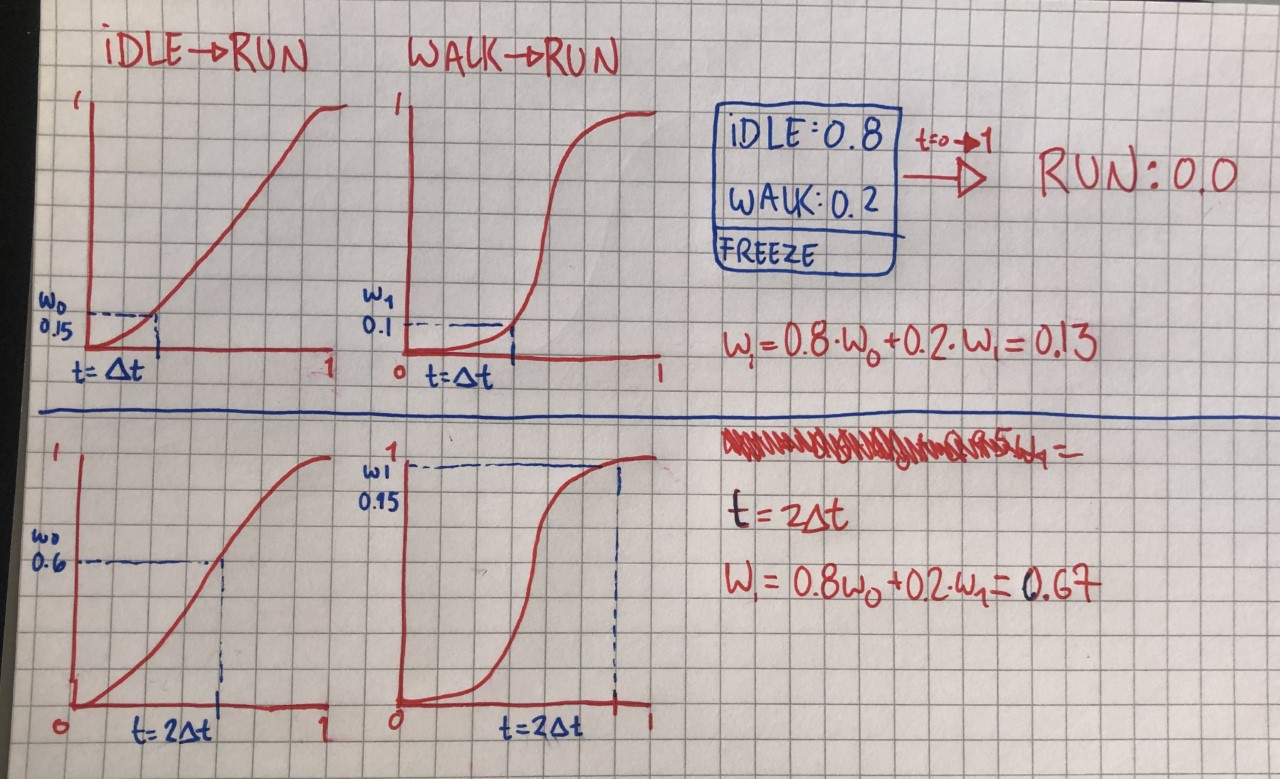
\includegraphics[width=\textwidth]{frozen-transitions}
  \caption{Frozen transition}
  \label{fig:frozen-transition}
\end{figure*}
To evaluate $step$ we notice that each $l\in\mathcal{L}$ should provide update routines $\dot{p}^*=l_p(\dot{p})$ and 

while the derivates can be used to update positions directly from dt to get the full actor update




velocity magnitude depends on the amount of turn.
Velocity direction is handeled by spring thing
orientation direction is handled by thing.
again each element could be an abitrarily complex sub system




velocity update depends and orientation relative to forward. And Also to rate of change of orientation.

Velocity springs towards target with crititically damped spring. exponential curve
orientation springs towards target 

Updates to the model is handled by the integration routine $p^*,q^*=I(m,C,p,q)$, and all $m_i,m_j\in\mathcal{M}$ are associated with a transition curve used to update $\vec{m}^*=T(C,\vec{m})$, ie., the update that handles transition times between movement modes. 
Each mode is associated with internal update procedures
\begin{equation}
\begin{split}
    p^*&=P(p,p',q')\\
    q^*&=Q(q,q',p')\\
\end{split}
\end{equation}
The update up the model is determined by the contribution of each movement mode in 
\begin{equation}
\begin{split}
    p^*&=\sum_{m\in{M}}{P_m*\vec{m}_m}\\
    q^*&=\sum_{m\in{M}}{Q_m*\vec{m}_m}\\
\end{split}
\end{equation}

Missing: Parameters exposed by P and Q update functions
Missing: Updates to velocities
Missing: Clear description of entire parameter set
Missing: Control signal could also contain

Notice that the formulation for $D$ is generic. In production a mapping between the generic movement model and a more context specific model would usually be needed. 

\subsection{missing}
Add animator constraint to model ? Example is 180. We dont start moving backwards immediately. First we rotate 90 degrees on the spot and then we start a 90 degree run to idle movement

Show very clear example. Pseudo code with idle and walk state. 